\documentclass[class={IEEEtran}]{standalone}
\usepackage{fontawesome7}
\usepackage{tikz}
\usepackage{amsmath}
\usepackage{pgf}
\usepackage{pifont}
\usepackage{xcolor}
\usepackage{contour}
\usepackage{mathptmx}

\contourlength{1pt} 
\pagestyle{empty}
\usetikzlibrary{shapes.geometric,shapes.arrows,positioning,calc,arrows.meta,math,backgrounds}

% --------- DEFINE COLORS ---------
% Blue 系
\definecolor{blue}{RGB}{76,114,176}        % 沉稳学术蓝
\definecolor{navy}{RGB}{59,72,99}           % 深藏青
\definecolor{steelblue}{RGB}{102,139,171}   % 钢蓝

% Red 系
\definecolor{red}{RGB}{180,82,82}           % 暗红（非警告型）
\definecolor{maroon}{RGB}{128,70,70}        % 学术酒红
\definecolor{brick}{RGB}{150,90,75}         % 砖红

% Green 系
\definecolor{green}{RGB}{90,140,120}        % 灰绿色
\definecolor{olive}{RGB}{120,130,90}        % 橄榄绿
\definecolor{forest}{RGB}{80,110,95}        % 深林绿

% Yellow / Orange 系
\definecolor{orange}{RGB}{200,140,90}       % 低饱和橙
\definecolor{goldenrod}{RGB}{170,145,85}    % 学术金
\definecolor{sand}{RGB}{190,175,140}        % 沙色

% Purple 系
\definecolor{purple}{RGB}{130,110,150}      % 灰紫
\definecolor{plum}{RGB}{120,95,125}         % 李子紫
\definecolor{violet}{RGB}{145,130,170}      % 冷紫

% Gray 系（强烈推荐学术使用）
\definecolor{gray}{RGB}{130,130,130}
\definecolor{darkgray}{RGB}{90,90,90}
\definecolor{lightgray}{RGB}{200,200,200}
% ---------------------------------
% ---- DEFINE GLOBAL VARIABLES ----
\newcommand{\AGENTSPAN}{0.2\textwidth}
\newcommand{\LINEHEIGHT}{3.2ex}
\newcommand{\ENDWIDTH}{1.4em}
\newcommand{\ENDHEIGHT}{0.4ex}
\newcommand{\LABELSIZE}{1}
\newcommand{\LABELCOLOR}{black}
% ---------------------------------
% --------- DEFINE STYLES ---------
\tikzset{AGENT/.style={rectangle,minimum width=5em,minimum height=3.5ex,draw,semithick,align=flush center, anchor=north,fill=white}}
\tikzset{ACTION/.style={rectangle,rounded corners,draw,semithick,align=flush left,fill=white}, anchor=north}
\tikzset{LABEL/.style={circle, draw, semithick, align=center, minimum size=1.2em, inner sep=0pt,fill=white}, anchor=north}
\tikzset{PREPARATION/.style={rectangle,draw,semithick,align=flush center,fill=white,dashed, anchor=north}}

% 基础单向箭头
\tikzset{Arrow/.style={thick, -stealth}}
% 基础单向箭头（细）
\tikzset{ArrowThin/.style={->,>=stealth, thin}}
% 加粗单向箭头
\tikzset{ArrowThick/.style={->,>=stealth, very thick}}
% 虚线箭头（流程/假设）
\tikzset{ArrowDash/.style={->,>=stealth, dashed, thick}}
% 点线箭头（弱关系）
\tikzset{ArrowDot/.style={->,>=stealth, dotted, thick}}
% 双向箭头
\tikzset{BiArrow/.style={<->,>=latex, thick}}
% 超粗双向箭头（强调用）
\tikzset{BiArrowThick/.style={<->,>=latex, very thick}}

\tikzset{LineThin/.style={thin}}
\tikzset{LineThick/.style={thick}}
\tikzset{LineDashed/.style={dashed, thin}}
\tikzset{LineDotted/.style={dotted, thick}}
% ---------------------------------
% -------- DEFINE COMMANDS --------
\newcommand{\NewCoord}[2]{\coordinate (#1) at (#2)}
\newcommand{\NewCoordRightToC}[3]{\coordinate (#1) at ($(#2)+(#3,0)$)}
\newcommand{\NewCoordBelowToC}[3]{\coordinate (#1) at ($(#2)+(0,-#3)$)}
\newcommand{\NewCoordRightToN}[3]{\coordinate (#1) at ($(#2.east |- #2.north)+(#3,0)$)}
\newcommand{\NewCoordBelowToN}[3]{\coordinate (#1) at ($(#2.south)+(0,-#3)$)}
\newcommand{\NewCoordAlignToN}[3]{\coordinate (#1) at ($(#3 -| #2.north)$)}

\newcommand{\NewNode}[4]{\node[#1] (#2) at (#3) {#4}}
\newcommand{\NewAgent}[3]{\node[AGENT] (#1) at (#2) {#3}}
\newcommand{\NewAction}[3]{\node[ACTION] (#1) at (#2) {#3}}
\newcommand{\NewLabel}[3]{\node[LABEL, scale=\LABELSIZE, text=\LABELCOLOR, draw=\LABELCOLOR] (#1) at (#2) {#3}}

\newcommand{\DrawLine}[3]{\draw[#1] (#2) -- (#3)}
\newcommand{\DrawArrow}[4]{\draw[#1] (#2) -- (#3) node[midway,above=-3pt]{\contour{white}{#4}}}

\makeatletter
\newcommand{\GetLowestCoord}[2]{%
    \global\pgf@ya=999pt%
    \def\pgf@lowest{(0,0)}%
    \foreach \p in {#2} {%
        \pgfextracty{\pgf@yb}{\pgfpointanchor{\p}{center}}%
        \ifdim\pgf@yb<\pgf@ya
          \global\pgf@ya=\pgf@yb
          \xdef\pgf@lowest{\p}%
        \fi
    }%
    \coordinate (#1) at (\pgf@lowest)
}
\makeatother

\newcommand{\DrawEnd}[2] {
  \NewCoordBelowToC{end_#1}{#2-|#1}{\LINEHEIGHT/2};
  \draw[semithick] (#1.south) -- (end_#1);
  \draw[fill=black] ($(end_#1)+(-\ENDWIDTH,0)$) rectangle ($(end_#1)+(\ENDWIDTH,-\ENDHEIGHT)$);
}
% ---------------------------------

\renewcommand{\AGENTSPAN}{0.145\textwidth}

\begin{document}
\begin{tikzpicture}

% ========================================
%   Agents
% ========================================
\NewCoord{c_U}{0,0};
\NewAgent{agent_U}{c_U}{\hspace{-0.5em} \faUser \; U};

\NewCoordRightToC{c_MW}{c_U}{\AGENTSPAN*1.35};
\NewAgent{agent_MW}{c_MW}{\hspace{-0.5em} \faBasketShopping \; MW};

\NewCoordRightToC{c_MS}{c_MW}{\AGENTSPAN*1.35};
\NewAgent{agent_MS}{c_MS}{\hspace{-0.5em} \faServer \; MS};

\NewCoordRightToC{c_WPS}{c_MS}{\AGENTSPAN*1.35};
\NewAgent{agent_WPS}{c_WPS}{\hspace{-0.5em} \faSackDollar \; WPS};

% ========================================
%   Messages
% ========================================

% Phase 1: Ordering
% -------------- Divide Line --------------
  \NewCoordRightToC{c_tmp}{agent_U.south}{-\AGENTSPAN/2};
  \NewCoordBelowToC{c_ldiv_1}{c_tmp}{\LINEHEIGHT/2};
  \NewCoordAlignToN{c_tmp}{agent_WPS}{c_ldiv_1};
  \NewCoordRightToC{c_rdiv_1}{c_tmp}{\AGENTSPAN/2};
  \DrawLine{LineDotted}{c_ldiv_1}{c_rdiv_1};
% ----------------------------------------
% ---------------- Label -----------------
  \NewCoordBelowToC{c_tmp}{c_ldiv_1}{\LINEHEIGHT*1.8};
  \NewCoordRightToC{c_label_1}{c_tmp}{1em};
  \NewLabel{label_1}{c_label_1}{\romannumeral 1};
% ----------------------------------------

\NewCoordBelowToC{c_act_U1}{c_ldiv_1-|c_U}{\LINEHEIGHT/2};
\NewAction{action_U1}{c_act_U1}{Select $goods$};

\NewCoordBelowToN{c_smsg_U_MW_1}{action_U1}{\LINEHEIGHT};
\NewCoordAlignToN{c_rmsg_U_MW_1}{agent_MW}{c_smsg_U_MW_1};
\DrawArrow{Arrow}{c_smsg_U_MW_1}{c_rmsg_U_MW_1}{$goods$};

\NewCoordBelowToC{c_smsg_MW_MS_1}{c_rmsg_U_MW_1}{\LINEHEIGHT/2};
\NewCoordAlignToN{c_rmsg_MW_MS_1}{agent_MS}{c_smsg_MW_MS_1};
\DrawArrow{Arrow}{c_smsg_MW_MS_1}{c_rmsg_MW_MS_1}{$goods$};

% Phase 2: Prepayment
% -------------- Divide Line --------------
  \NewCoord{c_tmp}{c_rmsg_MW_MS_1 -| c_ldiv_1};
  \NewCoordBelowToC{c_ldiv_2}{c_tmp}{\LINEHEIGHT/2};
  \NewCoordAlignToN{c_tmp}{agent_WPS}{c_ldiv_2};
  \NewCoordRightToC{c_rdiv_2}{c_tmp}{\AGENTSPAN/2};
  \DrawLine{LineDotted}{c_ldiv_2}{c_rdiv_2};
% ----------------------------------------
% ---------------- Label -----------------
  \NewCoordBelowToC{c_tmp}{c_ldiv_2}{\LINEHEIGHT*10};
  \NewCoordRightToC{c_label_2}{c_tmp}{1em};
  \NewLabel{label_2}{c_label_2}{\romannumeral 2};
% ----------------------------------------

\NewCoordBelowToC{c_act_MS1}{c_ldiv_2-|c_MS}{\LINEHEIGHT/2};
\NewAction{action_MS1}{c_act_MS1}{
  $out\_trade\_no, nonce := random()$\\
  $amount, description := calculate(goods)$ \\
  $body := appid || mchid || description || nonce $\\
  \quad\quad\quad $ || out\_trade\_no || notify\_url || amount$\\
  $S_{body} := sign_{priv_{M}}(body)$\\
  $message := mchid || S_{body} || body$
};

\NewCoordBelowToN{c_smsg_MS_WPS_1}{action_MS1}{\LINEHEIGHT};
\NewCoordAlignToN{c_rmsg_MS_WPS_1}{agent_WPS}{c_smsg_MS_WPS_1};
\DrawArrow{Arrow}{c_smsg_MS_WPS_1}{c_rmsg_MS_WPS_1}{$message$};

\NewCoordBelowToC{c_act_WPS1}{c_rmsg_MS_WPS_1}{\LINEHEIGHT/2};
\NewAction{action_WPS1}{c_act_WPS1}{
  \textbf{if} $validate(message)$ \textbf{then}\\
  \quad $continue()$\\
  \textbf{else} $abort()$\\
  $h5\_url := random()$
};

\NewCoordBelowToN{c_smsg_WPS_MS_1}{action_WPS1}{\LINEHEIGHT};
\NewCoordAlignToN{c_rmsg_WPS_MS_1}{agent_MS}{c_smsg_WPS_MS_1};
\DrawArrow{Arrow}{c_smsg_WPS_MS_1}{c_rmsg_WPS_MS_1}{$h5\_url$};

\NewCoordBelowToC{c_smsg_MS_MW_1}{c_rmsg_WPS_MS_1}{\LINEHEIGHT};
\NewCoordAlignToN{c_rmsg_MS_MW_1}{agent_MW}{c_smsg_MS_MW_1};
\DrawArrow{Arrow}{c_smsg_MS_MW_1}{c_rmsg_MS_MW_1}{$h5\_url$};

\NewCoordBelowToC{c_smsg_MW_WPS_1}{c_rmsg_MS_MW_1}{\LINEHEIGHT};
\NewCoordAlignToN{c_rmsg_MW_WPS_1}{agent_WPS}{c_smsg_MW_WPS_1};
\DrawArrow{Arrow}{c_smsg_MW_WPS_1}{c_rmsg_MW_WPS_1}{$h5\_url$};

% Phase 3: Payment
% -------------- Divide Line --------------
  \NewCoord{c_tmp}{c_rmsg_MW_WPS_1 -| c_ldiv_1};
  \NewCoordBelowToC{c_ldiv_3}{c_tmp}{\LINEHEIGHT/2};
  \NewCoordAlignToN{c_tmp}{agent_WPS}{c_ldiv_3};
  \NewCoordRightToC{c_rdiv_3}{c_tmp}{\AGENTSPAN/2};
  \DrawLine{LineDotted}{c_ldiv_3}{c_rdiv_3};
% ----------------------------------------
% ---------------- Label -----------------
  \NewCoordBelowToC{c_tmp}{c_ldiv_3}{\LINEHEIGHT*3};
  \NewCoordRightToC{c_label_3}{c_tmp}{1em};
  \NewLabel{label_3}{c_label_3}{\romannumeral 3};
% ----------------------------------------

\NewCoordBelowToC{c_smsg_WPS_U_1}{c_ldiv_3-|c_WPS}{\LINEHEIGHT};
\NewCoordAlignToN{c_rmsg_WPS_U_1}{agent_U}{c_smsg_WPS_U_1};
\DrawArrow{Arrow}{c_smsg_WPS_U_1}{c_rmsg_WPS_U_1}{$amount, description, account, ...$};

\NewCoordBelowToC{c_act_U_2}{c_rmsg_WPS_U_1}{\LINEHEIGHT/2};
\NewAction{action_U2}{c_act_U_2}{Enter $password$};

\NewCoordBelowToN{c_smsg_U_WPS_1}{action_U2}{\LINEHEIGHT/2};
\NewCoordAlignToN{c_rmsg_U_WPS_1}{agent_WPS}{c_smsg_U_WPS_1};
\DrawArrow{Arrow}{c_smsg_U_WPS_1}{c_rmsg_U_WPS_1}{$password$};

\NewCoordBelowToC{c_act_WPS2}{c_rmsg_U_WPS_1}{\LINEHEIGHT/2};
\NewAction{action_WPS2}{c_act_WPS2}{
  \textbf{if} validate($password$) \textbf{then} \\
  \quad $make\_payment()$\\
  \textbf{else} $abort()$
};

% Phase 4: Notification 
% -------------- Divide Line --------------
  \NewCoord{c_tmp}{action_WPS2.south -| c_ldiv_1};
  \NewCoordBelowToC{c_ldiv_4}{c_tmp}{\LINEHEIGHT/2};
  \NewCoordAlignToN{c_tmp}{agent_WPS}{c_ldiv_4};
  \NewCoordRightToC{c_rdiv_4}{c_tmp}{\AGENTSPAN/2};
  \DrawLine{LineDotted}{c_ldiv_4}{c_rdiv_4};
% ----------------------------------------
% ---------------- Label -----------------
  \NewCoordBelowToC{c_tmp}{c_ldiv_4}{\LINEHEIGHT*6};
  \NewCoordRightToC{c_label_4}{c_tmp}{1em};
  \NewLabel{label_4}{c_label_4}{\romannumeral 4};
% ----------------------------------------

\NewCoordBelowToC{c_act_WPS3}{c_ldiv_4-|c_WPS}{\LINEHEIGHT/2};
\NewAction{action_WPS3}{c_act_WPS3}{
  $id, transaction\_id, summary := random()$\\
  $nonce_{1}, nocne_{2} := random()$\\
  $data := appid || mchid || out\_trade\_no $\\
  \quad\quad\quad $|| transaction\_id || amount || nonce_{1}$\\
  $E_{data} := enc_{APIV3}(data)$\\
  $result := id || nonce_{1} || summary || nonce_{2}|| E_{data}$\\
  $S_{result} := sign_{priv_{W}}(result)$
};

\NewCoordBelowToN{c_smsg_WPS_U_2}{action_WPS3}{\LINEHEIGHT};
\NewCoordAlignToN{c_rmsg_WPS_U_2}{agent_U}{c_smsg_WPS_U_2};
\DrawArrow{Arrow}{c_smsg_WPS_U_2}{c_rmsg_WPS_U_2}{
  $\text{``Successful''}, amount, description, ...$
};

\NewCoordBelowToC{c_smsg_WPS_MS_1}{c_smsg_WPS_U_2}{\LINEHEIGHT};
\NewCoordAlignToN{c_rmsg_WPS_MS_1}{agent_MS}{c_smsg_WPS_MS_1};
\DrawArrow{Arrow}{c_smsg_WPS_MS_1}{c_rmsg_WPS_MS_1}{$result, S_{result}$};

\NewCoordBelowToC{c_act_MS3}{c_rmsg_WPS_MS_1}{\LINEHEIGHT/2};
\NewAction{action_MS3}{c_act_MS3}{
  \textbf{if} validate($result$) \textbf{then} \\
  \quad $continue()$\\
  \textbf{else} $abort()$
};

\NewCoordBelowToN{c_smsg_MS_WPS_2}{action_MS3}{\LINEHEIGHT};
\NewCoordAlignToN{c_rmsg_MS_WPS_2}{agent_WPS}{c_smsg_MS_WPS_2};
\DrawArrow{Arrow}{c_smsg_MS_WPS_2}{c_rmsg_MS_WPS_2}{
  $\text{``Successful''}$
};

% -------------- Divide Line --------------
  \NewCoord{c_tmp}{c_rmsg_MS_WPS_2 -| c_ldiv_1};
  \NewCoordBelowToC{c_ldiv_5}{c_tmp}{\LINEHEIGHT/2};
  \NewCoordAlignToN{c_tmp}{agent_WPS}{c_ldiv_5};
  \NewCoordRightToC{c_rdiv_5}{c_tmp}{\AGENTSPAN/2};
  \DrawLine{LineDotted}{c_ldiv_5}{c_rdiv_5};
% ----------------------------------------

% ========================================
%   Ends
% ========================================
\begin{scope}[on background layer]
  \GetLowestCoord{c_lowest}{c_ldiv_5};
  \DrawEnd{agent_U}{c_lowest};
  \DrawEnd{agent_MW}{c_lowest};
  \DrawEnd{agent_MS}{c_lowest};
  \DrawEnd{agent_WPS}{c_lowest};
\end{scope}

\end{tikzpicture}
\end{document}
